\subsection{DB Implementering}

Der er i projektets backend oprettet klasser, models, tilsvarende ER diagrammerne. Udover det valgte atributter er der også oprettet navigationals i de nødvendige klasse så der kan laves relationer.
Til implementering af databasen og opsætning af entiteter benytter vi Entity framework core. Opsætning af keys og relationer er lavet med EF cores fluent api, som gør det nemt og overskueligt.
På figur xx herunder ses opsætningen af keys for de forskellige entiteter. Disse er opsat efter ER diagrammerne på figur xx og xx.\\

\begin{figure}[H]
\centering
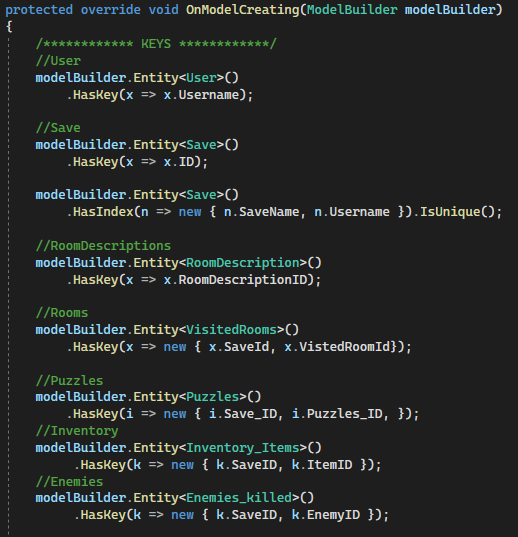
\includegraphics[width = 0.7\textwidth]{02-Body/Images/DAL-Database/DbKeys.PNG}
\caption{}
\label{fig:DbKeys}
\end{figure}

Udover de forskellige keys, skal der også opsætte relationer mellem de forskellige entiteter, som vist på figur xx og xx, med referencer til foreign keys. 
Opsætningen kan ses på figur xx herunder: 

\begin{figure}[H]
\centering
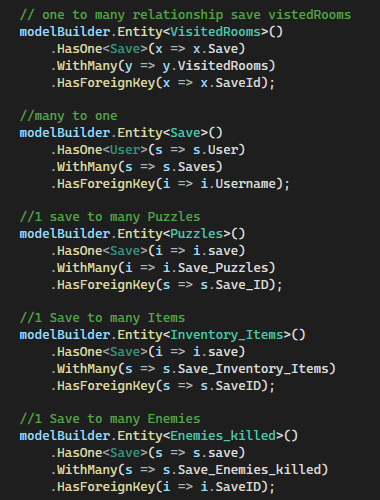
\includegraphics[width = 0.5\textwidth]{02-Body/Images/DAL-Database/DbRelations.PNG}
\caption{}
\label{fig:DbRelations}
\end{figure}

Databasen er på forhånd seedet med en enkelt bruger, ”Gamer1”, med password ”123”, som hashes ind i databasen. Gamer1 får derudover også 5 tilhørende "tomme" saves og til slut er der indsat rumbeskrivelser for hver af de 20 rum. Dette ses på figur xx herunder. \\

\begin{figure}[H]
\centering
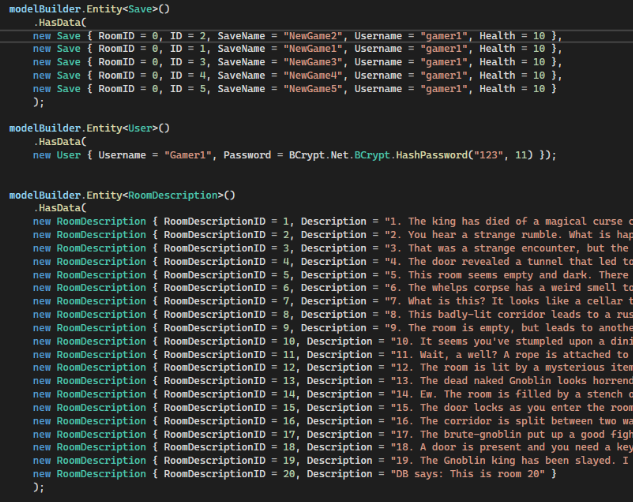
\includegraphics[width = \textwidth]{02-Body/Images/DAL-Database/DbSeeding.PNG}
\caption{}
\label{fig:DbSeeding}
\end{figure}